
\documentclass[
	oneside,
	12pt,				% tamanho da fonte
	%%openright,			% capítulos começam em pág ímpar (insere página vazia caso preciso)
	%%twoside,			% para impressão em recto e verso. Oposto a oneside
	a4paper,			% tamanho do papel. 
	english,			% idioma adicional para hifenização
	brazil,				% o último idioma é o principal do documento
	article
	]{abntex2}

% ---
% Pacotes fundamentais 
% ---

\usepackage{times}				% Usa a fonte Time News Roman
\usepackage[T1]{fontenc}		% Selecao de codigos de fonte.
\usepackage[utf8]{inputenc}		% Codificacao do documento (conversão automática dos acentos)
\usepackage{indentfirst}		% Indenta o primeiro parágrafo de cada seção.
\usepackage{microtype} 			% para melhorias de justificação
\usepackage{setspace}
\usepackage{graphicx}			% para o uso de imagens
\usepackage{float}
\usepackage{fancyhdr}
\pagestyle{fancyplain}
\fancyhf[]{}
\rfoot{\thepage}



% Pacotes de citações
% ---
\usepackage[brazilian,hyperpageref]{backref}	 % Paginas com as citações na bibl
\usepackage[alf]{abntex2cite}	% Citações padrão ABNT

\instituicao{UNIVERSIDADE FEDERAL DOS VALES DO JEQUITINHONHA E MUCURI - UFVJM
	PROGRAMA DE PÓS-GRADUAÇÃO STRICTO SENSU EM EDUCAÇÃO}
\titulo{Modelo de Ambiente Virtual de Aprendizado suportado por CS}
\local{Brasil}
\data{2019}

\renewcommand{\imprimircapa}{%
	\begin{capa}%
		\center	
		{\ABNTEXchapterfont\imprimirinstituicao}
		\vfill
		\begin{center}
			\ABNTEXchapterfont\bfseries\imprimirtitulo
		\end{center}
		\vspace*{3cm}
		\begin{flushright}
		Linha de pesquisa: EDUCAÇÃO E TECNOLOGIAS APLICADAS EM INSTITUIÇÕES EDUCACIONAIS.
		\linebreak
		Possível Orientador: Prof. Dr. Cristiano Grijó Pitangui
		\end{flushright}
		\vfill
		\imprimirlocal 
		\linebreak		
		\imprimirdata
		\vspace*{1cm}
	\end{capa}
}

% informações do PDF
\makeatletter
\hypersetup{
     	%pagebackref=true,
		pdftitle={\@title}, 
		pdfauthor={\@author},
    	pdfsubject={\imprimirpreambulo},
	    pdfcreator={LaTeX with abnTeX2},
		pdfkeywords={abnt}{latex}{abntex}{abntex2}{projeto de pesquisa}, 
		colorlinks=true,       		% false: boxed links; true: colored links
    	linkcolor=blue,          	% color of internal links
    	citecolor=blue,        		% color of links to bibliography
    	filecolor=magenta,      		% color of file links
		urlcolor=blue,
		bookmarksdepth=4
}


% O tamanho do parágrafo é dado por:
\setlength{\parindent}{1.3cm}
% Controle do espaçamento entre um parágrafo e outro:
\setlength{\parskip}{0.2cm}  % tente também \onelineskip

% Configurações de margem do projeto
\usepackage[left=2.5cm, right=2.5cm, top=2.5cm, bottom=2.5cm]{geometry}



\begin{document}
 
% Seleciona o idioma do documento (conforme pacotes do babel)
%\selectlanguage{english}
\selectlanguage{brazil}

% Retira espaço extra obsoleto entre as frases.
\frenchspacing 

%% Imprimir capa via abntex
\imprimircapa

\textual

\OnehalfSpacing %%set espaçamento entre linhas de 1cm
\begin{center}
	\ABNTEXchapterfont\bfseries RESUMO
\end{center}

Consciência Situacional (CS) é amplamente utilizada na correta compreensão do ambiente e da situação, sendo considerada principal precursora do processo de Tomada de Decisão, portanto, considerando seu poder de compreensão do universo, a CS tem o potencial de ser aplicada em Ambientes Virtuais de Aprendizagem (AVA’s).
O Ambiente Educacional compõe-se de um espaço extremamente dinâmico, por tanto muitas vezes as inúmeras situações presentes em um estado podem dificultar o processo de tomada de decisão. Atualmente é notório o crescimento de pesquisas que baseiam-se no uso de Mineração de Dados Educacionais (MDE) afim de extrair conhecimento dos dados de AVA's, entretanto somente a MDE por vezes não é suficiente para lidar com a variedade de dados e eventos gerados da interação de cada usuário com o Ambiente Educacional. \citeonline{Martins2018} desenvolve um Modelo baseado em CS e Mineração de Dados Educacionais (MDE) de suporte a aprendizagem em AVA's, o modelo propõe a expansão da MDE através da CS utilizando-se de modelos mentais, indicando fortes benefícios ao ambiente escolar, entretanto o autor não aplica o modelo ainda no ambiente. Este projeto de pesquisa objetiva-se na expansão do modelo, o uso de ontologias para a construção de regras decisórias e modelos mentais demonstra-se viável para a aplicabilidade do problema, é necessário também a construção e teste do mesmo, assim a elaboração de um protótipo de software para aplicabilidade do modelo são objetivos deste projeto de pesquisa. Espera-se que este estudo permita a aplicabilidade do modelo de CS no âmbito educacional, procurando assim minimizar a sobrecarga de professores e tutores dentro do ambiente educacional, espera-se também observar uma nova perspectiva da MDE, visando atingir um níveis de CS em situações nas quais tais técnicas e procedimentos apresentam uma melhor performance. 
\linebreak\linebreak
\textbf{Palavras-chave:} Consciência da Situação. Ambientes Virtuais de Aprendizagem. Mineração de Dados Educacionais. 
\linebreak\linebreak
\textbf{TÍTULO:} Modelo de Ambiente Virtual de Aprendizado suportado por CS.


%\setSpacing{1.5} %%set espaçamento entre linhas de 1.5cm
\section{Introdução}

Modalidades de ensino por Educação à Distância (EaD) caracterizam práticas pedagógicas diferenciadas no processo de ensino e aprendizagem, de forma que tal modalidade utiliza-se das tecnologias de informação e comunicação visando facilitar a aquisição do conhecimento \cite{Rabelo_et_al2017}.

Ambientes Virtuais de Aprendizagem (AVA’s) reproduzem modelagens e instruções que possam inferir o estado do aprendizado de cada estudante, \citeonline{Rabelo_et_al2017} reiteram que essas plataformas suportam a interação entre alunos e o ambiente educacional, gerando assim valores expressivos de dados, estes quais quando gerenciados e analisados podem recomendar ampliações sobre os usuários e sua dinâmica de interação com o sistema.

\citeonline{Falci_et_al_2018} descrevem que o relacionamento entre professores e alunos nestas plataformas dá-se pela troca de materiais, discussão em fóruns e chats, todavia, estes meios por muitas vezes não são suficientes o bastante para que o discente possa extrair o máximo de conhecimento dos assuntos trabalhados.

A Mineração de Dados Educacionais (MDE) são a aplicação das técnicas de Mineração de Dados em dados oriundos de ambientes educacionais \cite{Romero_Ventura_2013}. \citeonline{Fernandes2017} reforça que o uso destas técnicas são soluções promissoras para a compreensão dos dados extraídos de AVA's. 

O conhecimento extraído do círculo educacional pode ser melhor utilizado a partir de análise consciente do ambiente educacional, \citeonline[p. 13]{Endsley2012} descrevem o entendimento dos sinais presentes em um ambiente de Consciência Situacional (CS). Estar ciente da situação deve ser um componente natural da organização cognitiva humana, e os benefícios que resultam de um melhor entendimento da situação podem ser percebidos desde a pré-história \cite{Roy_Breton_Rousseau_2007}.

\citeonline{Martins2018} propõe um modelo baseado em CS e MDE para o apoio ao ensino em Ambientes Virtuais de Aprendizagem, seu modelo usa aspectos da CS para otimizar a ação das técnicas de MDE sobre o conjunto de dados e posteriormente auxiliar o usuário na tomada de decisão via regras decisórias. Tomando base esta pesquisa, o foco deste trabalho concentra-se no estudo e expansão do modelo no uso de ontologias para a construção de novas regras decisórias e modelagens mentais assim como na criação de um protótipo de software para aplicabilidade do modelo.


\section{Objetivos}

\subsection{Objetivo Geral}

Esta pesquisa possui como objetivo geral a aplicação da CS em AVA's, investigar o uso de ontologias no modelo proposto por \citeonline{Martins2018}, validar e construir um software baseado no mesmo para teste e aplicação em mundo real.

\subsection{Objetivos Específicos}

\begin{itemize}
	\item Construção do software baseado no modelo para aplicação em dados reais;
	\item Aplicar o conceito de ontologia do módulo seletor do modelo;
	\item Avaliar os resultados da aplicação do modelo identificando como a CS pode entregar uma nova perspectiva para o usuário no momento da tomada de decisão.  
\end{itemize}

\section{Motivação e Caracterização do Problema de Pesquisa}

A sobrecarga de informações em um ambiente educacional inunda docentes e discente de dados e situações que devem ser avaliadas diariamente, pesquisas aprofundam-se na descoberta de conhecimento por meio da MDE, onde o uso de técnicas de processamento de dados e algoritmos aplicados resultam em conhecimento sobre aquela situação específica.

Apesar da MDE prover resultados satisfatórios quando aplicado em AVA's por vezes o uso dos algoritmos restringe-se a situação específica para a qual foi desenvolvida, nota-se então dentro da literatura a vasta abordagem sobre performances e execução dos algoritmos aplicado sobre o ambiente educacional em análises comparativas. 

O uso da Consciência Situacional procura dar uma nova perspectiva sobre o uso da MDE em AVA's, visto o grande uso de CS no auxílio de tomadas de decisão em situações críticas, o seu uso poderá contribuir significativamente nas definições de quais técnicas terão resultados mais expressivos quando aplicados naquela configuração de estados.

O modelo descrito por \citeonline{Martins2018} descreve como a CS e a MDE podem somar forças para potencializar os resultados dentro de um ambiente educacional, entretanto seu trabalho não passou de uma ideia, não sendo testado com dados reais. O autor ainda deixa aberto um leque de possibilidades que podem ser estudadas para utilização com a CS como o uso de ontologias. Deste modo, este trabalho busca resolver as seguintes questões:

\begin{itemize}	
	\item \textbf{Como pode ser expandido o modelo proposto por \citeonline{Martins2018}?;}
	\item \textbf{Este modelo realmente pode trazer benefícios quando aplicados a dados reais?.}	 
\end{itemize}

\section{Justificativa}

A presente proposta de pesquisa justifica-se por perceber o grande crescimento da modalidade de cursos de Educação a Distância (EAD), tal modalidade vem consolidando como importante ferramenta de capacitação independentemente de tempo e localização de seus usuários. Os AVA's podem gerar informações sobre o processo de aprendizagem do estudantes, resultados estes da análise dos dados decorrentes da interação do usuário com a plataforma \cite{Fernandes2017}.

\citeonline{Leite_et_al_2016} reforçam o uso de MDE como soluções promissoras para compreensão de informações nas base de dados em AVA’s, \cite{Rabelo_et_al2017} destacam o seu uso na descoberta de padrões e informações novas sobre conjuntos de dados relacionados aos ambientes de aprendizagem, suas estruturas e personagens.

\citeonline{Falci_et_al_2018} reitera que sistemas com técnicas de Inteligência Artificial (IA) podem facilitar a comunicação entre computador e estudante, permitindo a criação de ambientes com conteúdo adaptativo ao modelo cognitivo do aluno. 

Pesquisas focam na aplicação da CS em ambiente de características dinâmicas, processos estocásticos e eventualmente de resultados incertos, dado o comportamento humano com relevante grau de impacto ao sistema e pelo tempo como fator crítico de alto nível \cite{Berti2017}.

Dessa maneira, construir modelos de AVA's que utilizam tecnologias baseadas em MDE, CS e demais áreas relacionadas  a IA podem facilitar a tomada de decisão, potencializando o processo de aprendizagem, graças a geração de dados mais claros e assertivos que auxiliam o professor no correto entendimento do ambiente.


\section{Desenvolvimento Teórico}

Esta seção abordará o modelo conceitual e computacional proposto por \citeonline{Martins2018} e as definições de CS, MDE e Modelos Mentais necessárias para entendimento do modelo.

\subsection{Fundamentos Conceituais}

\cite [p. 97]{Endsley1988} define CS como: `` a percepção dos elementos no ambiente dentro de um volume de tempo e espaço, a compreensão dos seus significados, e a projeção dos seus estados em um futuro próximo ". \citeonline{Endsley1995} separa  a CS em: \textbf{(i)} a captação sinais do ambiente, variáveis relevantes, elementos e atributos do ambiente, é o primeiro passo para obtenção da Consciência Situacional {\textit{(Percepção)}, \textbf{(ii)} o estudo dos significados presentes nas relações e interações dos sinais e variáveis do ambiente \textit{(Compreensão)} e \textbf{(iii)} predição de estados futuros, ou seja, a antecipação dos prováveis eventos que ocorrerão na sequência das próximas ações \textit{(Projeção)}.  

Modelos Mentais são: `` mecanismos pelos quais humanos são capazes de gerar descrições e formas de sistemas propostos, explicações de funcionalidades e estados observados do sistema, e previsões de estados futuros " \cite[p.60]{Rouse1985} apud \cite{Endsley1995}. A mente humana capta o mundo exterior a partir de representações mentais \cite{Moreira1996}. Um indivíduo  possui dois tipos de memórias: \textbf{(i)} a \textit{memória de trabalho} é pequena e uma pessoa deve relacionar-se ativamente com as informações para não esquecê-las, \textbf{(ii)} \textit{memórias de longo-prazo} são o conhecimento consolidado em estruturas bem definidas na mente \cite{Endsley2012}.

A MDE são os usos das técnicas de Mineração de Dados voltadas ao contexto educacional \cite{Leite_et_al_2016},  \cite{Romero_Ventura_2013}. \citeonline{Garcia_et_al_2011} e \citeonline{Santos2016} descrevem a MDE como uma conversão de dados brutos de Sistemas Educacionais em conhecimento útil para serem utilizadas por desenvolvedores de software, professores, pesquisadores educacionais e etc.

\subsection{Modelo Conceitual}

O Modelo Conceitual (figura \ref{modeloSAemAVA}) descreve o fluxo dos dados em uma representação alto-nível, os seus módulos aplicam-se diretamente na construção de representações sobre o conteúdo educacional. Os dados resultam-se do relacionamento entre Aluno X Professor X Banco de Dados Educacional, seguindo posteriormente para as etapas da CS.

Na percepção existe a coleta e o pré-processamento dos dados, na compreensão aplicam-se os algoritmo da MDE para a transformação de dados crus em informação útil e na projeção estruturas pré-definidas de modelos mentais antecipam quais estados futuros podem ser atingidos com as informações recebidas dos dados processados na etapa anterior.

\begin{figure}[H]	
	\centering
	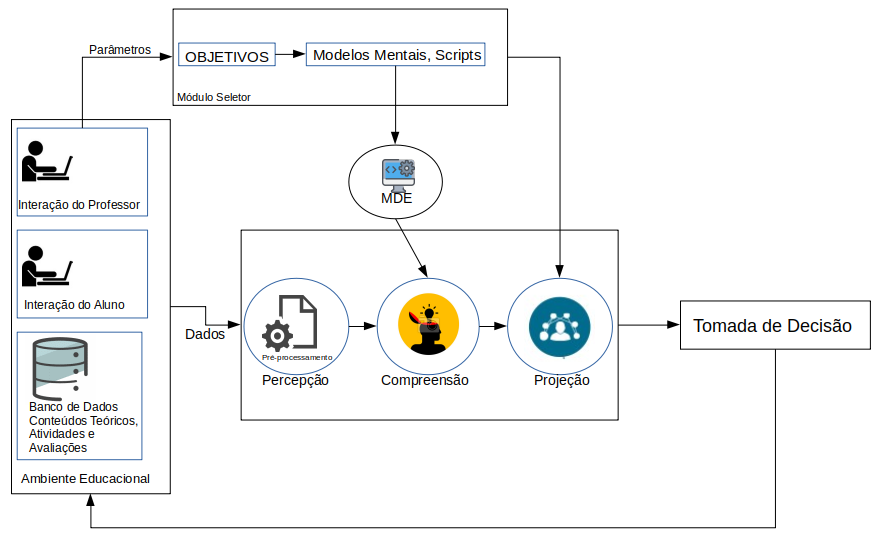
\includegraphics[scale=0.57]{teste_modelov02}
	\caption{Modelo de Apoio ao Ensino em Ambientes Virtuais de Aprendizagem sustentado por Consciência Situacional- Perspectiva Conceitual. Fonte: \cite{Martins2018} }
	\label{modeloSAemAVA}	
\end{figure}

O módulo seletor é uma transcrição os conhecimentos obtidos através de experiências prévias, construindo-se assim as estruturas de modelos e mapas mentais. Tais estruturas definem quais métodos devem ser utilizados diante de cada parâmetro de funcionamento no início de uma iteração, assim como qual algoritmo e construção mental aplicará-se melhor ao caso vigente no momento da iteração.

\subsection{Modelo Computacional}

O Modelo Computacional (figura \ref{modeloSAemAVAcomp}) é a representação lógico-computacional do Modelo Conceitual, estruturando os métodos e dados em uma arquitetura de processamento em máquina. A representação a seguir, compõe-se essencialmente de três blocos principais, sendo, Ambiente Educacional, Modelo Mental e Consciência Situacional.

O Ambiente Educacional assemelha-se muito com o do modelo conceitual abrigando o universo educacional, onde docentes e discentes são agentes/usuários que interagem com o sistema, e um Banco de Dados que abrange os conteúdos teóricos, atividades propostas e avaliações.

O módulo Consciência Situacional é onde trabalha-se diretamente com os dados para extração de conhecimento e projeção dos estados futuros, ele processa os dados conforme os métodos e técnicas definidos pelo módulo Modelo Mental.

\begin{figure}[H]	
	\centering
	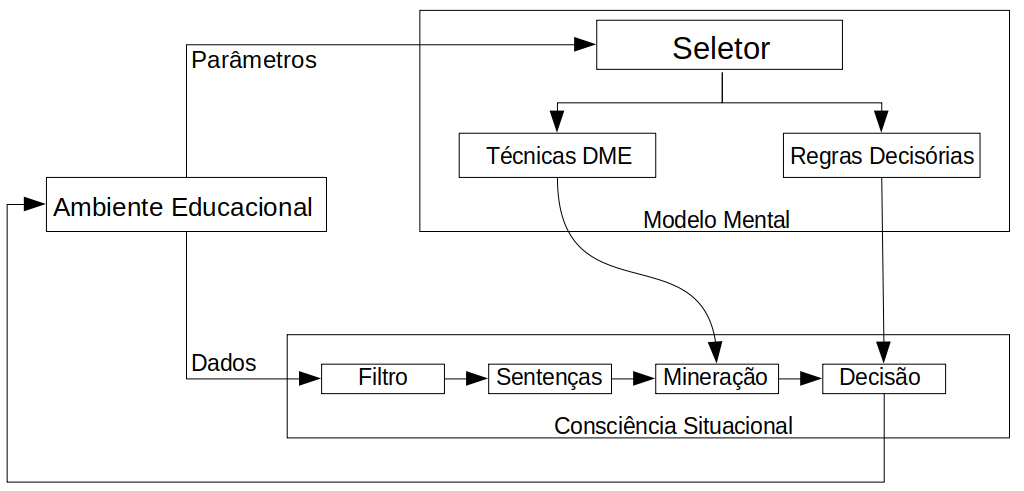
\includegraphics[scale=0.4]{modelo_persp_comp}
	\caption{Modelo de Apoio ao Ensino em Ambientes Virtuais de Aprendizagem sustentado por Consciência Situacional- Perspectiva Computacional. Fonte: \cite{Martins2018} }
	\label{modeloSAemAVAcomp}	
\end{figure}

O presente trabalho foca-se na expansão do módulo Modelo Mental, procurando assim novas formas de representação computacional do conhecimento. O módulo proposto por \citeonline{Martins2018} usa regras decisórias e árvores de decisão para estruturação do conhecimento.

\citeonline{Kokar2009} formalizam os principais conceitos da Consciência Situacional por meio de ontologias, definindo linguagens que sejam comumente suportadas por homens e computadores o autor utiliza-se de Linguagens de Ontologias Web. 

\citeonline{Kokar2009} descrevem ainda a captação de linguagens formais e a sua representação por meio da Teoria Ontológica da Situação providenciando assim uma semântica que recria fatos do mundo real nos termos ontológicos para que possam ser inferidos usando um motor de inferência. 

\citeonline{Garcia_et_al_2011} desenvolvem um modelo de seleção, construção e validação de regras designadas a educação. Sua pesquisa objetiva-se na construção de uma ferramente de EMD baseada em regras de associação que seja de fácil visualização e intuitiva a educadores, e agentes do ambiente educacional.
 
As pesquisas de \citeonline{Kokar2009} inspiram a expansão do modelo proposto por \citeonline{Martins2018} na criação de ontologias para o desenvolvimento de regras de inferência, e por sua vez \citeonline{Garcia_et_al_2011} influenciam e exemplificam a criação de um software com visualização sucinta e clara para os agentes do ambiente educacional.

\section{Procedimentos Metodológicos}

A presente pesquisa é do tipo quantitativa, exploratória, visto que pretende-se desenvolver e comparar métodos para estruturação de um modelo mental em AVA's e avaliar a possível contribuição de um software consciente da situação quando utilizados em ambientes educacionais.

A pesquisa iniciará com a criação de cenários de situações que circundam o ambiente educacional transcrevendo-se em regras ontológicas conforme descrito por \cite{Kokar2009}. Um exemplo de cenário poderia aplicar-se na seguinte configuração:

Cenário:
``O Professor está sobe atividades no AVA. Antônio um aluno aplicado, logo verifica quais as datas de entrega e aplica-se ao desenvolvimento dos exercícios, Maria apesar de boa aluna nunca acessa seu ambiente virtual assim que uma notificação nova aparece pois ela tem acesso ao ambiente geralmente aos finais de semana, por esta dificuldade Maria usa com muita Frequência os fóruns de discussão da plataforma para discutir com colegas e tirar dúvidas. Antônio prefere realizar as tarefas o mais rápido possível, não se atentando assim para as discussões em fóruns". 

Pode-se inferir desse cenário duas informações importantes sendo a velocidade de acesso e constância de uso da plataforma (Antônio) e utilização e participação nos fóruns de discussão (Maria). Tal cenário deve traduzir-se em um ontologia para que possa deduzir informações a partir de regras de inferência.

O passos seguintes dar-se-ão através da construção do protótipo de software do modelo de \cite{Martins2018}. Este protótipo será construído como uma aplicação web

\section{Possíveis Contribuições}



% ----------------------------------------------------------
% Referências bibliográficas
% ----------------------------------------------------------
\bibliography{library}

\end{document}